
\subsubsection*{Routing engine}
A key component of the TOTUS system is its routing engine. It enables some of the most powerful features in TOTUS like trip-dependent exposure and energy calculation as well as route optimisation based on arbitrary cost functions (e.g. minimum distance or energy). This module is implemented based on pgRouting (vXX\todo{pgRouting version?})\cite{dummy_temp}\todo{citation needed pgRouting}. The implementation of this module takes a streamlined version of the Open Street Map \cite{dummy_temp}\todo{OSM ref} data schema and converts it into a directed graph using \textit{osmosis}\cite{dummy_temp} and \textit{osm2pgrouting}\cite{dummy_temp}. The routing information is kept on a separate data schema that can be linked to the physical road network by the unique OSM feature identifier. From a scenario evaluation point of view, the advantages of the database routing approach for TOTUS are that the spatial data and attributes can be modified and any data changes can be reflected instantaneously through the routing engine. 

\subsubsection*{Exposure}
The current version of TOTUS' exposure module is based on a \textit{Traffic Impact Factor} developed by Longley et al\cite{dummy_temp}\todo{Citation needed TIF} to model $NO_2$ on a arbitrary grid covering a city. The method calculates, for a given point, an estimate of the traffic impact from all the roads in the domain. This is applied to the centre of the grid cells. The model is calibrated for a specific region using traffic data and $NO_2$ measurements. The following diagram describes the calculations. For more details see Longley et al\cite{dummy_temp}\todo{Citation needed TIF}

\begin{equation}
\label{eq:tif}
TIF_{x,y} = \sum_{road=1}^{R}{(Length_{road}*Traffic_{road})^{exp}}
\end{equation}
\todo[inline]{A DIAGRAM OF TIF}

\subsubsection*{Energy}

This module enables the implementation of an energy consumption calculator for any arbitrary census area (from meshblock to country) based on any layer available in the system. The implementation of the energy consumption model is flexible and allows for the interactive generation of various scenarios. 
\todo{Is this a generalised linear model?}
In simple terms, the module only stores the \textit{metadata} needed to configure a model run in terms of its identifier ( \textit{activity} and \textit{scenario}) and the specific model definition. The definition is stored in the \textit{model\_definition} table while \textit{model\_definition\_part} defines the individual terms of the formula (see Equation \ref{eq:energy}) that are aggregated to produce a final intensity
value. Each model definition part is described by a data field and the coefficient to apply. Figure \ref{fig:energy_diag} shows an overview of the Energy data schema.

\begin{equation}
\label{eq:energy}
EI=\sum_{parts}{CensusData_1*C_1+CensusData_2^{C_2}}
\end{equation}


\begin{figure}
	\caption{Energy schema overview}
	\label{fig:energy_diag}
	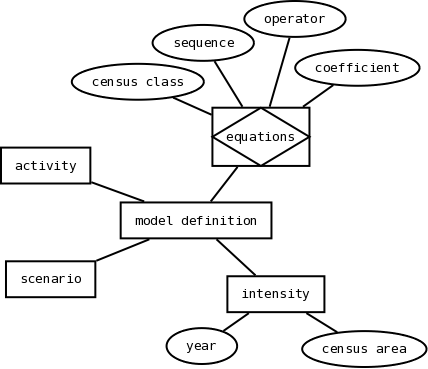
\includegraphics[width = 12cm]{energy.png}
\end{figure}

\subsubsection*{Emissions}
By extending the use of the \textbf{Energy} module, the Emissions and Socio-economic Model (ESESM)\todo{Wilton, E., Baynes, M., Bluett, J. (No date) Good practice guide for designing and implementing an incentive programme for domestic heating. Report prepared under the Envirolink Tools project nember NIWX0802, Environet and NIWA, 171p.} was implemented. The formulation\todo[inline]{This needs finishing ... describe what we did and how} as an extension of the \textbf{Energy} module is:

\begin{equation}
\label{eq:ESESM}
Emissions1 = Some definition
\end{equation}
